\section{Intégration et Expérimentations}\label{sec:ext:prefs:integration}
Dans cette section, nous présentons l'intégration de l'implémentation des opérateurs \textbf{Best/KBest} dans notre système Astronef-Asteroid. Tout d'abord, nous détaillons les règles qu'il est nécessaire de fournir à Astronef pour prendre en compte ces opérateurs. Puis, nous expérimentons les versions statiques et incrémentales de nos algorithmes afin de déterminer une \textit{heuristique} permettant de sélectionner le meilleur.

\subsection{Intégration dans Astronef}
Nous avons désormais des définitions Astral correctement posées. Nous pouvons maintenant intégrer ces opérateurs à Astronef. En premier lieu, nous avons conçu un composant opérateur capable de calculer les sémantiques de \textbf{Best} et \textbf{KBest} de manière statique en calculant à partir de l'état de $R(b)$. Ce composant prend évidemment en paramètre $k$ qui peut être égal à $-1$ pour indiquer une sémantique de \textbf{Best}.

L'intégration du composant se fait en deux parties. Tout d'abord, il est nécessaire d'enregistrer le composant en tant qu'opérateur\footnote{Cette opération est faite au moment de l'installation de l'extension dans Astronef.}. Ensuite, il faut renseigner ses définitions Astral dans le moteur de règle. Dans notre cas, quatre règles sont suffisantes :
\begin{lstlisting}
sugar([best,Config,C],[kbest,NewConfig,C]):-
    map_put(Config,['k',-1],NewConfig), !. % best = kbest avec k=-1

typerules([kbest,_,_,[T]],T):- relation(T), !.
attribrules([kbest,_,_,[A]], A):- !.

implrules([kbest,_,_,_], "KBest"):- !.
\end{lstlisting}

Une fois ce code renseigné dans le service \textit{KnowledgeBase} d'Astronef (présenté en~\ref{sec:contrib:astronef:integration}), nous pouvons librement utiliser les opérateurs \textbf{Best} et \textbf{KBest} sur toutes relations temporelles. Il est intéressant de voir que si le SGBD supporte le langage \textit{CPref-SQL}, nous pouvons pousser les opérateurs \textbf{Best} et \textbf{KBest} sur le SGBD via une règle Asteroid. 

\subsection{Expérimentations pour la sélection du plan de requête}
Nous avons à notre disposition deux composants capables de calculer de manière incrémentale ou non les opérateurs de préférences contextuelles. Dans cette section, nous expérimentons pour déterminer les cas où il est préférable de sélectionner l'un ou l'autre choix.

L'expérience a été réalisée dans un cadre applicatif financier. Ainsi, $30,000$ n-uplets ont été collectés depuis des flux de cours d'actions\footnote{Fournit par le service Dukascopy's Data Export. Disponible à \url{http://www.dukascopy.com/swiss/english/data_feed/csv_data_export}}. Les préférences utilisées sont de la même complexité que celles présentées en section~\ref{sec:ext:prefs:algo}, les détails sont présents dans notre papier~\cite{Petit:topk}. Soit $S$ un flux, la requête que nous analysons est la suivante : $${\bf KBest}_k(S[N \textrm{ slide } \Delta])$$

\begin{figure}[ht]
\subfigure[En variant $\Delta$ sur KBest (pour $N=500$)]{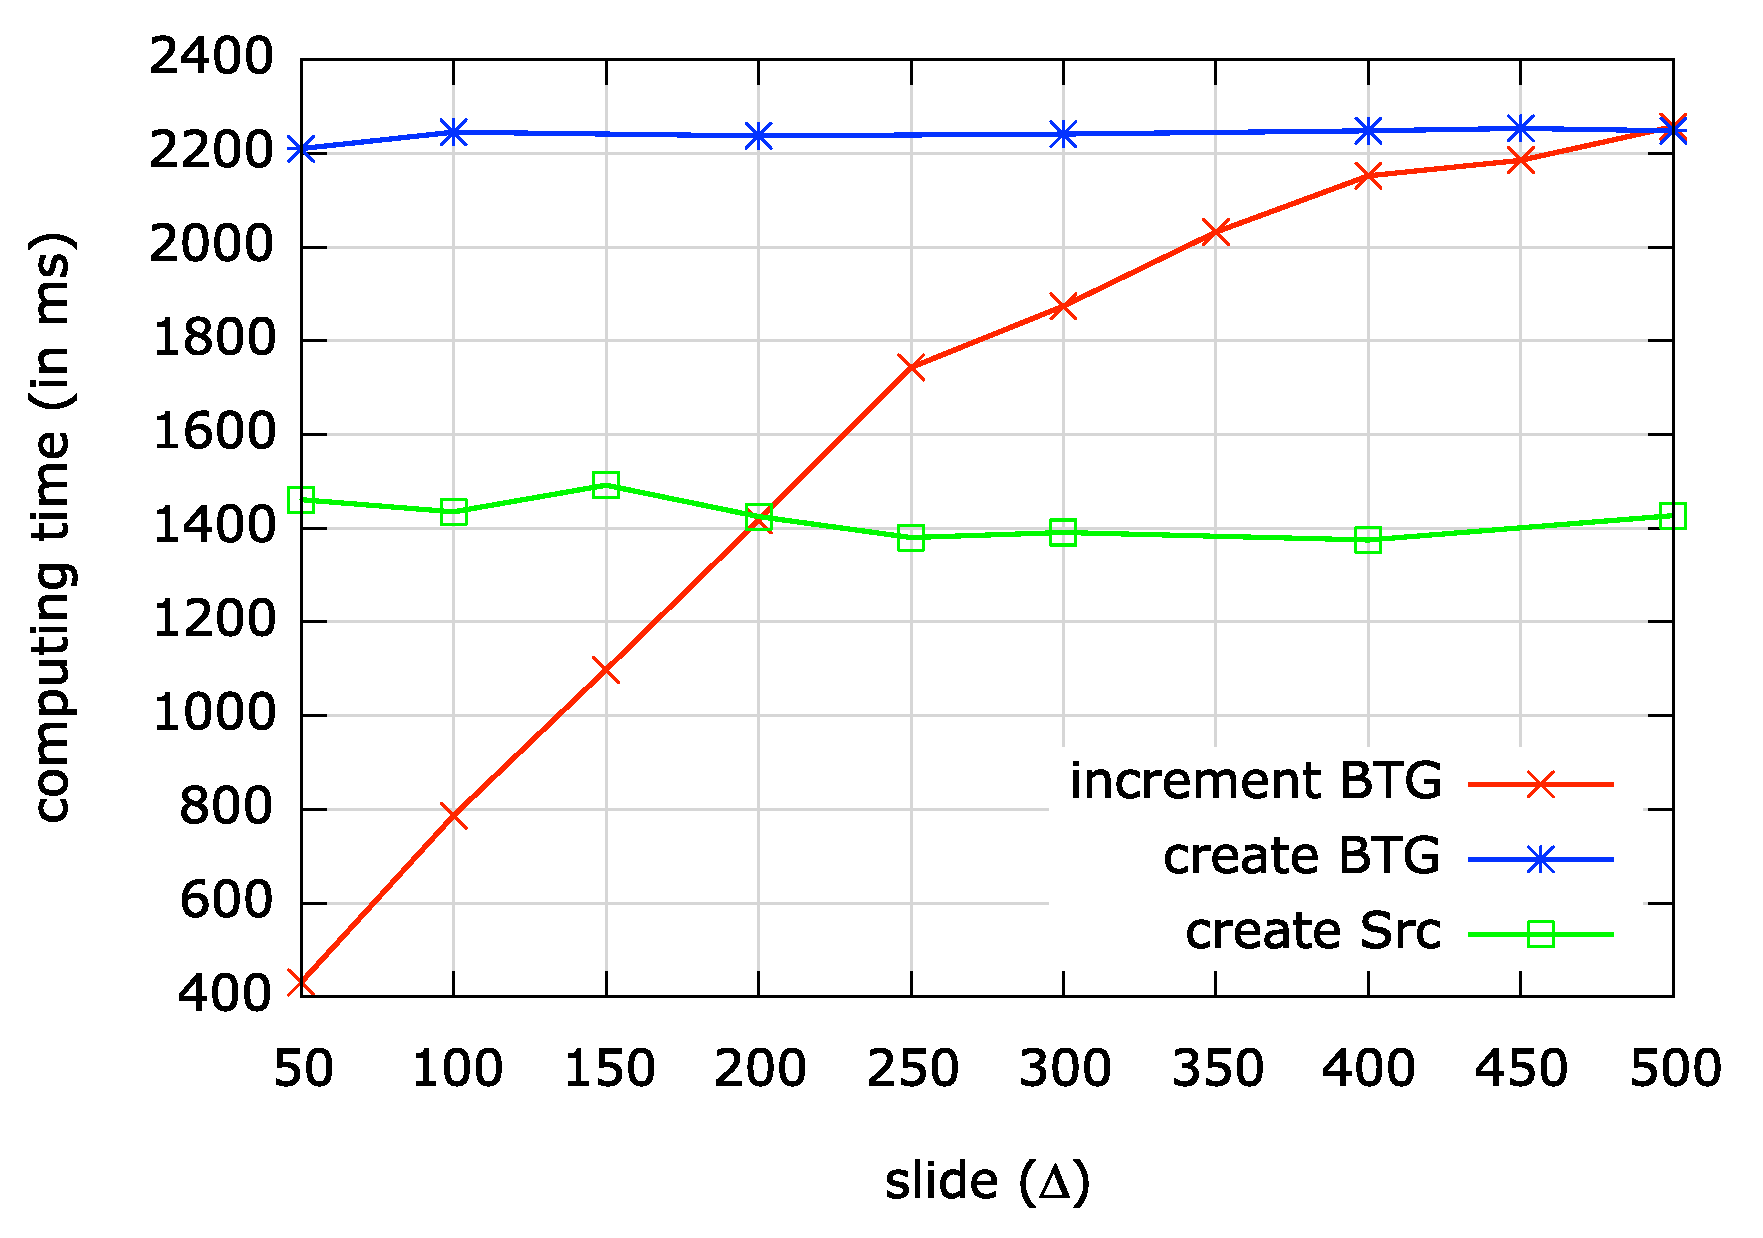
\includegraphics[width=0.48\linewidth]{valid-perfs-prefs-slide}\label{fig:prefxp-slide}}
\subfigure[En variant $N$ sur KBest (pour $\Delta=N$)]{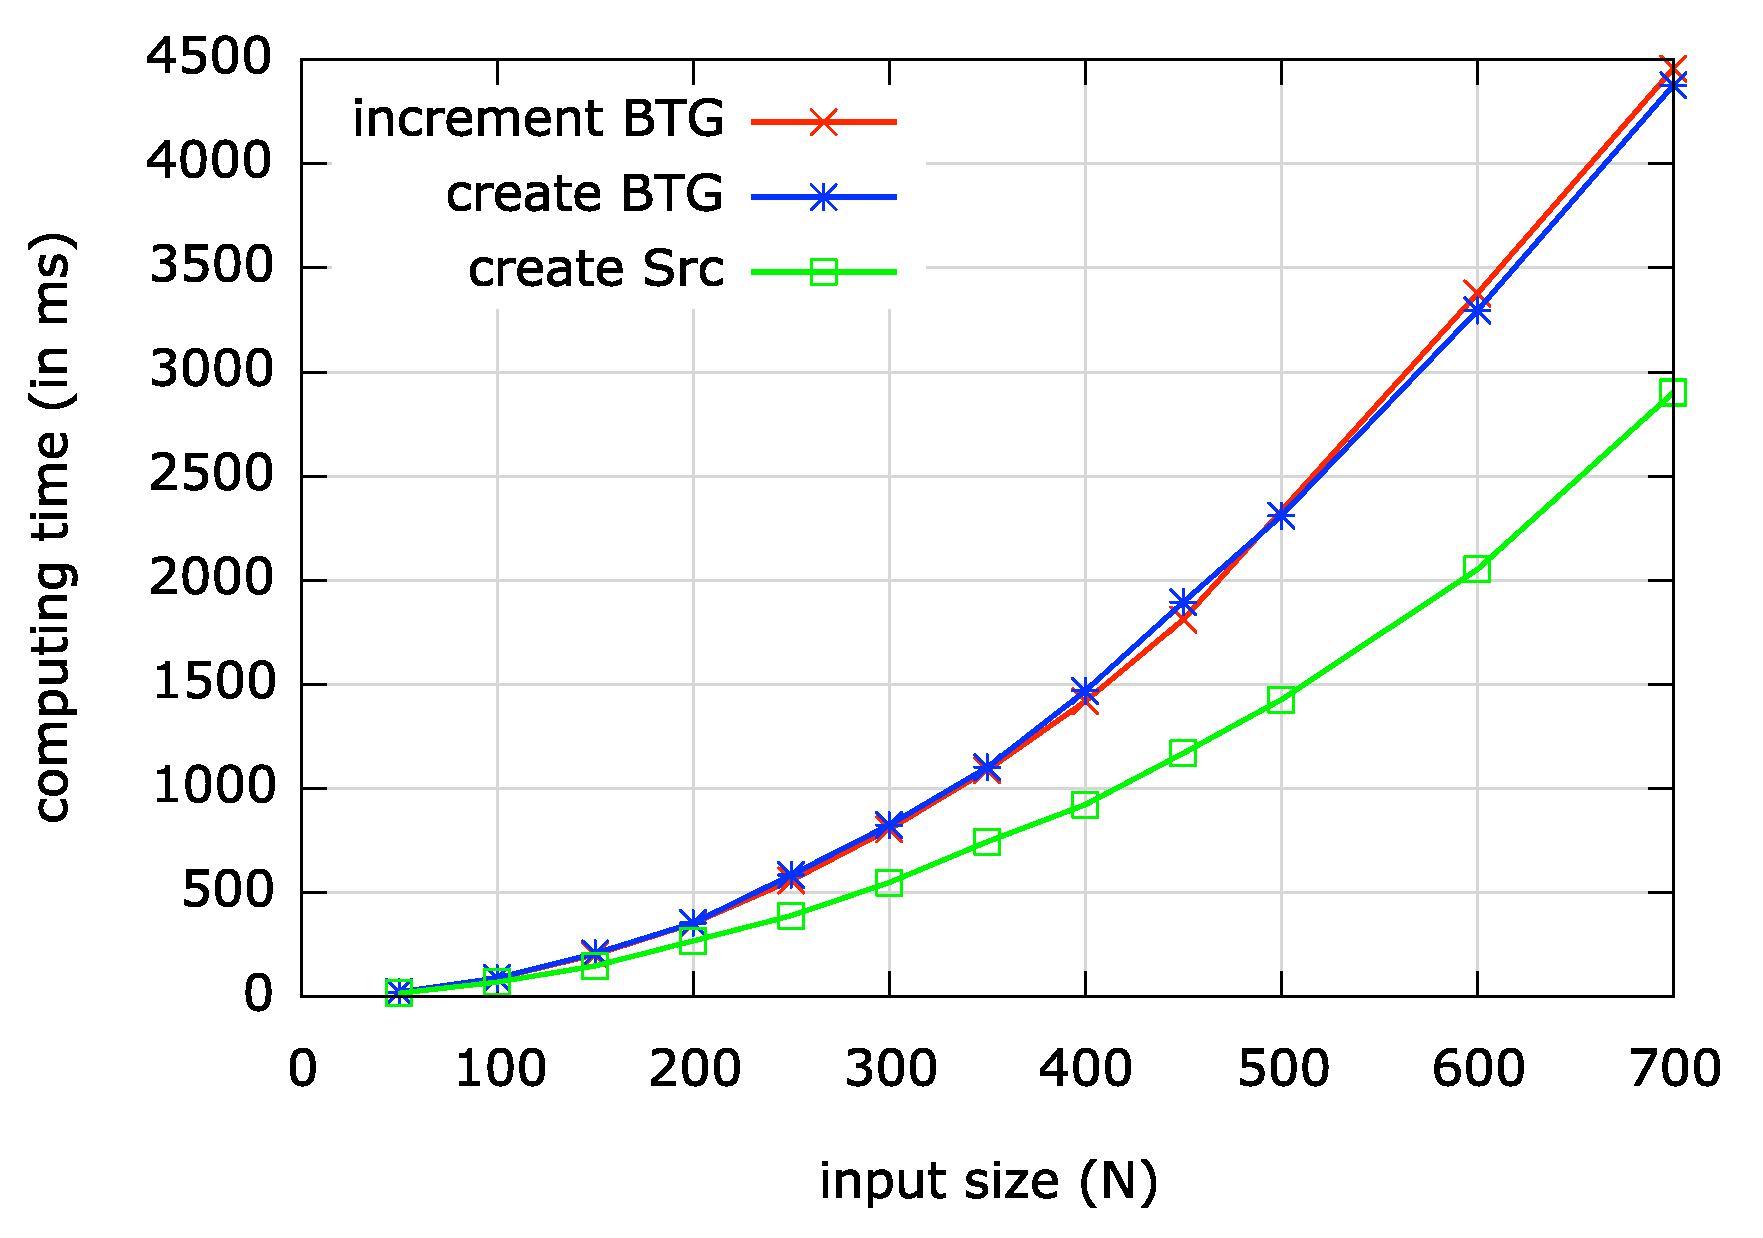
\includegraphics[width=0.48\linewidth]{valid-perfs-prefs-size}\label{fig:prefxp-size}}
\caption{Temps de calcul de \textit{Créer GP}, \textit{GP Incrémental} et de la maintenance de \textit{Src}}\label{fig:prefxp}
\end{figure}

\textbf{Résultats :} Les expérimentations montrent que le temps d'évaluation de \textbf{KBest} est dominé par la construction-mise à jour du \textit{GP}. Nous avons aussi observé que la structure du \textit{GP} d'une fenêtre à l'autre pouvait changer. La profondeur maximale du graphe varie de 2 à 6 et le nombre de n-uplets non-dominés varie de $1$ à $N$. Les grands changements de structures correspondent aux pires cas de l'algorithme incrémental. La figure~\ref{fig:prefxp-slide} montre le temps de calcul des deux algorithmes du \textit{GP} : \textit{créer} et \textit{incrémental}. Elle indique aussi le temps nécessaire au calcul réduit de la maintenance de \textit{Src}, qui est directement utilisée pour l'opérateur \textbf{Best}. 

Durant les expérimentations, nous avons utilisé plusieurs tailles de fenêtres $N$ et de taux $\Delta$. Nous remarquons que les changements de taux de mise à jour n'impactent pas le temps de création du \textit{GP}, tandis que l'algorithme incrémental obtient un gain de 6 pour un ration $N/\Delta=10$. Étonnement, les deux algorithmes du \textit{GP} se comportent de la même façon lorsque $\Delta\sim N$, ce qui correspond au cas où il n'y aurait pas ou peu d'intersections entre les fenêtres successives. Cela indique que dans la version incrémentale, les suppressions dans le \textit{BTG} prennent peu de temps comparé aux insertions. Ceci est notamment dû au fait que l'insertion nécessite l'évaluation des comparaisons (coûteuses dans notre cadre expérimental). Le coût de ces suppressions peut aussi être augmenté dans le cas où le \textit{GP} est un graphe fortement connexe, ce qui est difficile à trouver dans la pratique.

La variation de la taille de la fenêtre (figure~\ref{fig:prefxp-size} avec $\Delta=N$) montre que le comportement n'est pas impacté par le nombre de n-uplets impliqués. Comme prévu, l'évolution semble quadratique selon $N$ et l'approche incrémentale suit strictement la performance de l'algorithme de création.

Nous pouvons désormais intégrer notre composant incrémental à l'intérieur d'Astronef par la création de la règle suivante :
\begin{lstlisting}[language=PrologAstral]
implrules([kbest,B,[C]], "DynamicKBest"):- 
    map_get(B, "incremental", "true", "true"), % Mode incremental par defaut
    dynamicoperator(C), !. % Si le noeud fils est aussi incremental
\end{lstlisting}
Pour plus de complétude, nous pourrions établir une règle disant que si nous sommes dans le cas $k=-1$ (i.e. \textbf{Best}) et que le ratio $N/\Delta$ de la description de fenêtre, s'il y en a une, est inférieur à 2 : alors nous devons utiliser l'opérateur \textbf{Best} non-incrémental.
